\subsection{Artifacts}
\label{sec:appendix-artifacts}
The modified version of OpenHands that was used can be found at \url{\OpenHandsArtifactURL}. The full set of trajectories and generated apps for the models can be found here: \url{\VCBTrajectoriesURL}. The example specification, UI tests, and prompt for the harness are in Appendices \ref{sec:appendix-spec-example}, \ref{sec:appendix-ui-test-example}, and \ref{sec:generation-prompt}.

\subsection{Pass-Rate Histograms for All Models}
\label{sec:appendix-pass-rate-histograms}

\begin{figure}[!h]
\centering
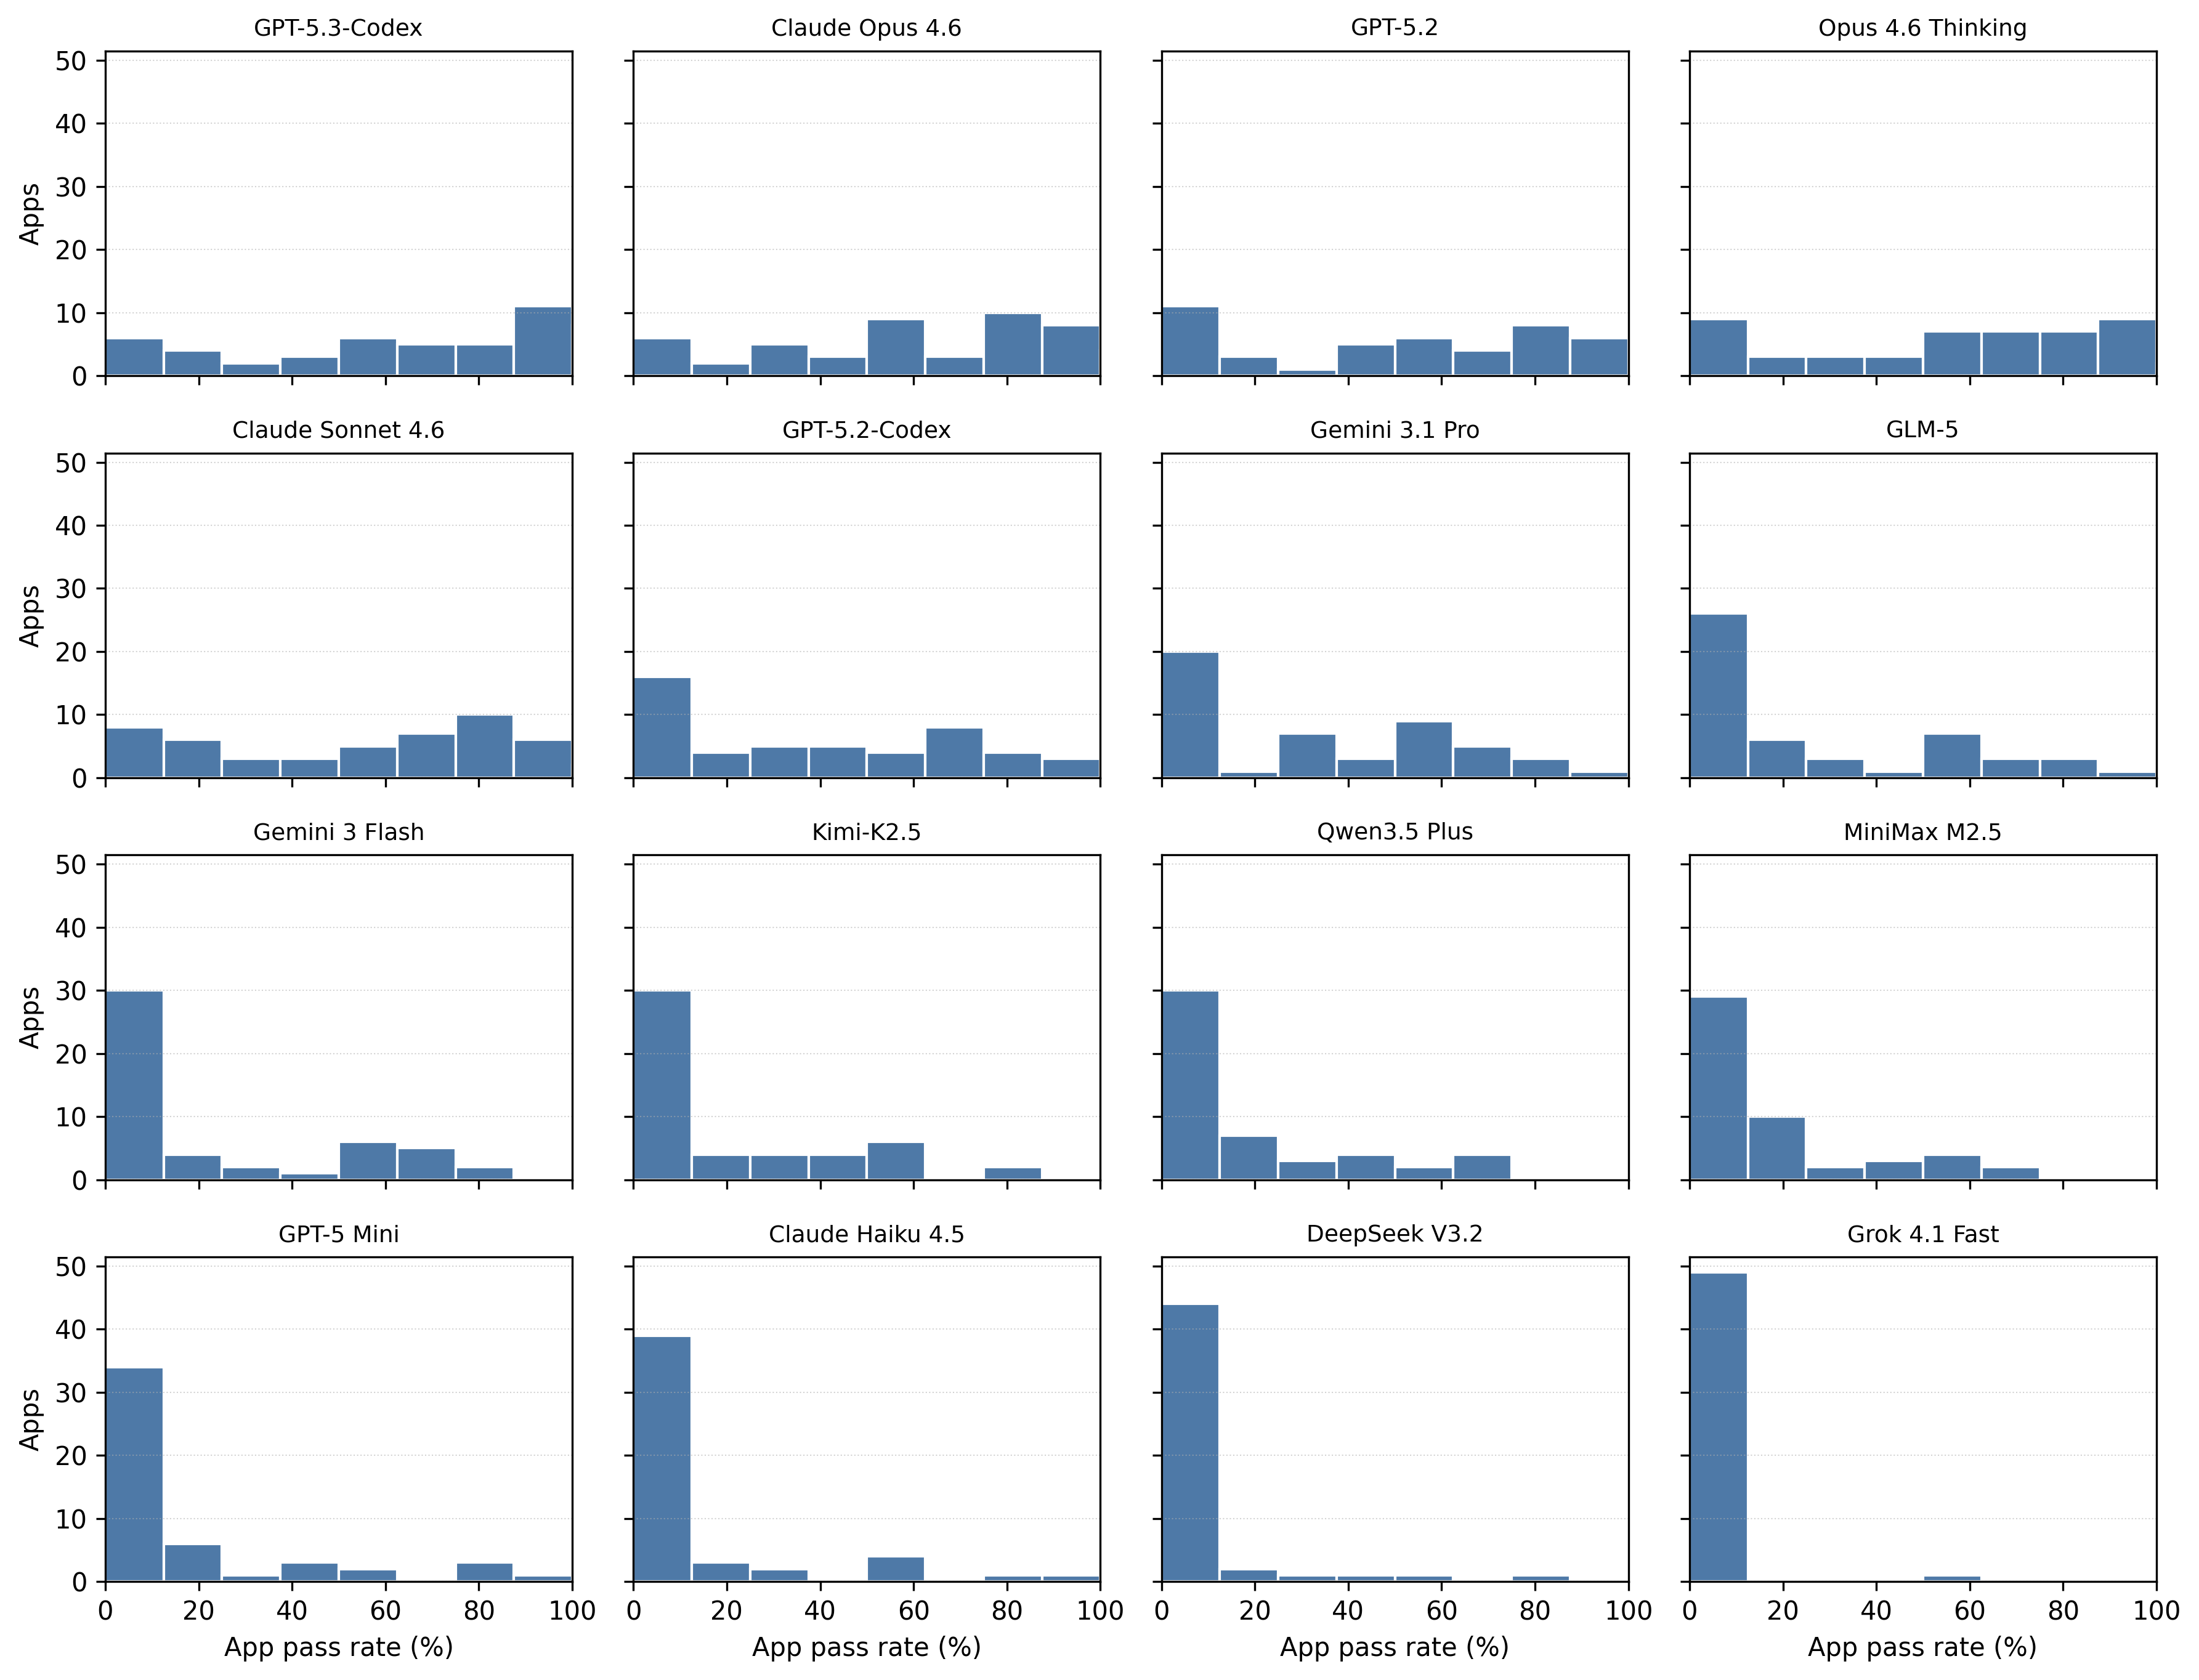
\includegraphics[width=0.98\textwidth]{pass_rate_hist_all_models_appendix.png}
\caption{Application pass-rate histograms for all evaluated models (test split).}
\label{fig:pass_rate_hist_all_models}
\Description{Grid of histograms, one per model, showing counts of application pass rates across 12.5-point bins.}
\end{figure}

\clearpage
\subsection{Illustrative Single-App Trajectories}
\label{sec:appendix-trajectory-example}
Figure~\ref{fig:trajectory_profiles} shows the rollout of a trajectory on a single application. Unlike Figure \ref{fig:trajectory_action_composition}, it is organized chronologically.

\begin{figure}[!h]
\centering
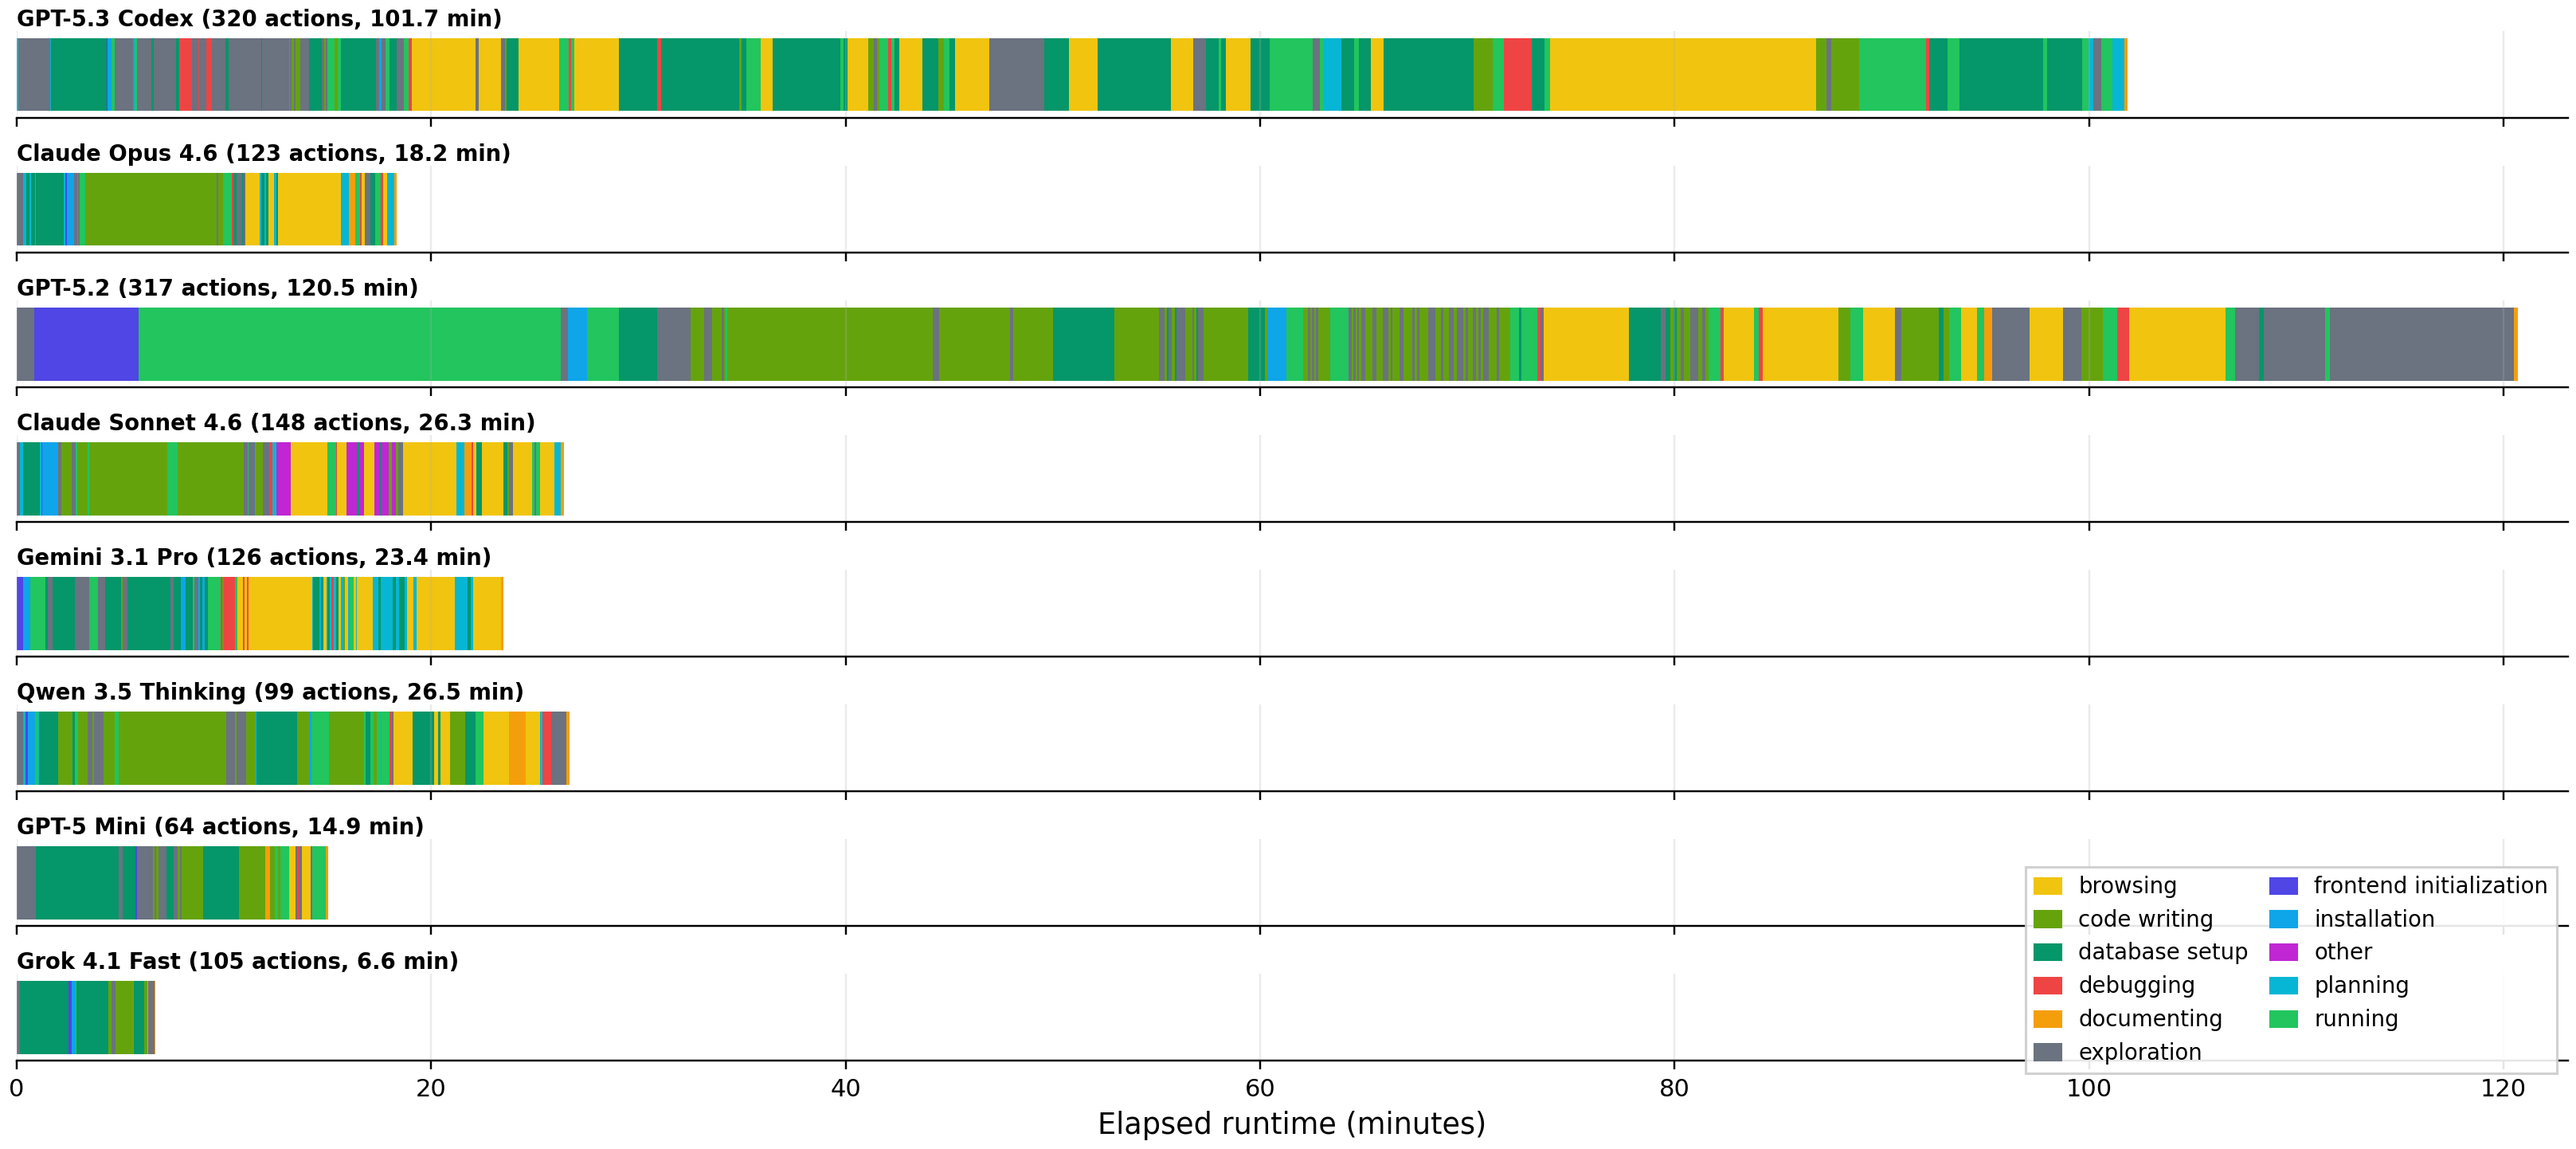
\includegraphics[width=0.98\textwidth]{trajectory_timescale.png}
\caption{Trajectory timeline by model on a single application (\texttt{bill\_splitting\_app}).}
\label{fig:trajectory_profiles}
\Description{Time-aligned action timelines across eight models, where each colored segment is one categorized agent action over elapsed runtime.}
\end{figure}

\subsection{All-Model Breakdown Results}
\label{sec:all_model_slice_appendix}
Tables~\ref{tab:all_model_difficulty_appendix}, \ref{tab:all_model_integration_appendix}, and \ref{tab:all_model_domain_appendix} extend the main difficulty, integration, and domain analyses to all 16 evaluated models. 

\begin{table}[!h]
\centering
\caption{All-model accuracy by difficulty (\%).}
\label{tab:all_model_difficulty_appendix}
\small
\setlength{\tabcolsep}{2pt}
\renewcommand{\arraystretch}{0.9}
\begin{tabular}{@{}lrrr@{}}
\toprule
\textbf{Model} & \textbf{Easy} & \textbf{Med.} & \textbf{Hard} \\
\midrule
GPT-5.3-Codex & 81.88 & 57.91 & 13.13 \\
Claude Opus 4.6 & 73.20 & 54.11 & 20.86 \\
GPT-5.2 & 81.53 & 33.72 & 19.88 \\
Opus 4.6 Thinking & 71.67 & 46.49 & 17.91 \\
Claude Sonnet 4.6 & 69.19 & 46.61 & 12.13 \\
GPT-5.2-Codex & 58.97 & 26.62 & 4.18 \\
Gemini 3.1 Pro & 46.24 & 28.33 & 0.00 \\
GLM-5 & 40.51 & 12.43 & 0.00 \\
Gemini 3 Flash & 34.21 & 10.32 & 3.41 \\
Kimi-K2.5 & 27.07 & 12.32 & 2.50 \\
Qwen3.5 Plus & 31.71 & 3.03 & 0.00 \\
MiniMax M2.5 & 29.37 & 3.53 & 0.00 \\
GPT-5 Mini & 27.99 & 2.35 & 2.50 \\
Claude Haiku 4.5 & 22.53 & 2.70 & 0.00 \\
DeepSeek V3.2 & 10.02 & 1.32 & 0.00 \\
Grok 4.1 Fast & 2.61 & 0.00 & 0.00 \\
Avg. Model & 44.29 & 21.36 & 6.03 \\
\bottomrule
\end{tabular}
\end{table}

\begin{table}[!h]
\centering
\caption{All-model accuracy by integration (\%).}
\label{tab:all_model_integration_appendix}
\small
\setlength{\tabcolsep}{2pt}
\renewcommand{\arraystretch}{0.9}
\begin{tabular}{@{}lrrrr@{}}
\toprule
\textbf{Model} & \textbf{None} & \textbf{Email} & \textbf{Stripe} & \textbf{Both} \\
\midrule
GPT-5.3-Codex & 71.25 & 55.00 & 12.50 & 29.58 \\
Claude Opus 4.6 & 63.58 & 46.25 & 25.00 & 41.59 \\
GPT-5.2 & 60.63 & 50.62 & 31.25 & 23.81 \\
Opus 4.6 Thinking & 60.58 & 31.25 & 37.50 & 33.37 \\
Claude Sonnet 4.6 & 59.41 & 38.12 & 25.00 & 24.73 \\
GPT-5.2-Codex & 44.15 & 24.38 & 12.50 & 19.95 \\
Gemini 3.1 Pro & 38.42 & 32.50 & 12.50 & 3.57 \\
GLM-5 & 27.60 & 23.12 & 0.00 & 7.74 \\
Gemini 3 Flash & 22.05 & 33.75 & 0.00 & 8.46 \\
Kimi-K2.5 & 20.44 & 10.00 & 12.50 & 7.94 \\
Qwen3.5 Plus & 19.75 & 11.25 & 0.00 & 1.59 \\
MiniMax M2.5 & 18.74 & 5.00 & 0.00 & 4.17 \\
GPT-5 Mini & 18.07 & 10.00 & 0.00 & 0.00 \\
Claude Haiku 4.5 & 14.31 & 0.00 & 0.00 & 5.75 \\
DeepSeek V3.2 & 6.23 & 0.00 & 0.00 & 3.57 \\
Grok 4.1 Fast & 1.62 & 0.00 & 0.00 & 0.00 \\
Avg. Model & 34.18 & 23.20 & 10.55 & 13.49 \\
\bottomrule
\end{tabular}
\end{table}

\begin{table}[!h]
\centering
\caption{All-model accuracy by domain (\%).}
\label{tab:all_model_domain_appendix}
\small
\setlength{\tabcolsep}{2pt}
\renewcommand{\arraystretch}{0.9}
\begin{tabular}{@{}lrrr@{}}
\toprule
\textbf{Model} & \textbf{Individual} & \textbf{Solo Founder} & \textbf{Enterprise Tool} \\
\midrule
GPT-5.3-Codex & 76.93 & 62.50 & 49.39 \\
Claude Opus 4.6 & 56.59 & 63.09 & 50.73 \\
GPT-5.2 & 72.53 & 56.50 & 35.11 \\
Opus 4.6 Thinking & 57.94 & 61.79 & 38.77 \\
Claude Sonnet 4.6 & 73.46 & 51.30 & 35.24 \\
GPT-5.2-Codex & 45.27 & 43.06 & 25.31 \\
Gemini 3.1 Pro & 49.30 & 37.07 & 12.16 \\
GLM-5 & 44.24 & 21.58 & 10.14 \\
Gemini 3 Flash & 29.01 & 21.79 & 11.41 \\
Kimi-K2.5 & 34.00 & 11.68 & 13.24 \\
Qwen3.5 Plus & 34.17 & 13.99 & 4.32 \\
MiniMax M2.5 & 30.82 & 14.61 & 3.22 \\
GPT-5 Mini & 37.85 & 5.91 & 7.77 \\
Claude Haiku 4.5 & 26.50 & 11.44 & 0.00 \\
DeepSeek V3.2 & 14.54 & 2.67 & 1.39 \\
Grok 4.1 Fast & 5.00 & 0.00 & 0.00 \\
Avg. Model & 43.01 & 29.94 & 18.64 \\
\bottomrule
\end{tabular}
\end{table}

\clearpage

\subsection{Tools Provided}
\label{sec:provided-tools}
\begin{table}[!h]
\begin{subtable}{\textwidth}
\centering
\caption{OpenHands tools (7).}
\label{tab:tools-openhands}
\small
\begin{tabular}{@{}llp{8.5cm}@{}}
\toprule
\textbf{\#} & \textbf{Tool Name} & \textbf{Description} \\
\midrule
1  & \texttt{execute\_bash}          & Execute a bash command in a persistent shell session. Supports chaining, background processes, interactive input, and configurable timeouts. \\
2  & \texttt{browser}                & Interact with a web page via 15 browser actions: navigate, click, fill, scroll, hover, press, select option, double-click, focus, clear, drag-and-drop, upload file, go back/forward, and wait. \\
3  & \texttt{str\_replace\_editor}   & View, create, and edit files. Commands: \texttt{view}, \texttt{create}, \texttt{str\_replace}, \texttt{insert}, \texttt{undo\_edit}. Requires exact string matching for replacements. \\
4  & \texttt{execute\_ipython\_cell} & Run Python code in an IPython environment with persistent variables and \texttt{\%pip} magic support. \\
5  & \texttt{think}                  & Log a reasoning step for planning and brainstorming. Does not execute code or produce side effects. \\
6  & \texttt{finish}                 & Signal task completion with a summary message; ends the interaction. \\
7  & \texttt{task\_tracker}          & Structured task management. Commands: \texttt{view} (show task list) and \texttt{plan} (create/update tasks with status tracking). \\
\bottomrule
\end{tabular}
\end{subtable}

\vspace{1em}

\begin{subtable}{\textwidth}
\centering
\caption{Supabase Studio MCP tools (11).}
\label{tab:tools-supabase}
\small
\begin{tabular}{@{}llp{8.5cm}@{}}
\toprule
\textbf{\#} & \textbf{Tool Name} & \textbf{Description} \\
\midrule
1  & \texttt{execute\_sql}                & Execute a raw SQL query against the Postgres database. Intended for DML and one-off statements. \\
2  & \texttt{apply\_migration}            & Apply a DDL migration with version tracking. Requires a snake\_case name and a SQL query. \\
3  & \texttt{list\_tables}                & List all tables in one or more schemas (defaults to \texttt{public}). \\
4  & \texttt{list\_extensions}            & List all installed Postgres extensions. \\
5  & \texttt{list\_migrations}            & List all previously applied migrations. \\
6  & \texttt{get\_logs}                   & Fetch logs by service type (api, postgres, auth, storage, realtime, edge-function, branch-action) from the last 24 hours. \\
7  & \texttt{get\_advisors}               & Retrieve security or performance advisory notices (e.g.\ missing RLS policies). \\
8  & \texttt{get\_project\_url}           & Return the API URL for the Supabase project. \\
9  & \texttt{get\_anon\_key}              & Return the anonymous API key for the project. \\
10 & \texttt{generate\_typescript\_types} & Generate TypeScript type definitions from the database schema. \\
11 & \texttt{search\_docs}               & Search the Supabase documentation via a GraphQL query. Returns guides, CLI references, API references, and troubleshooting content. \\
\bottomrule
\end{tabular}
\end{subtable}

\vspace{1em}

\begin{subtable}{\textwidth}
\centering
\caption{Tavily MCP tools (4).}
\label{tab:tools-tavily}
\small
\begin{tabular}{@{}llp{8.5cm}@{}}
\toprule
\textbf{\#} & \textbf{Tool Name} & \textbf{Description} \\
\midrule
1  & \texttt{tavily-search}  & Real-time web search with customizable depth, domain filtering, time-range filtering, and support for general and news topics. Returns titles, URLs, content snippets, and optional images. \\
2  & \texttt{tavily-extract} & Extract and process content from specified URLs with basic or advanced parsing modes, including tables and embedded content. \\
3  & \texttt{tavily-crawl}   & Systematically crawl websites starting from a base URL with configurable depth, breadth limits, domain filtering, and path pattern matching. \\
4  & \texttt{tavily-map}     & Create structured site maps by analyzing website structure and navigation paths. Supports configurable depth, domain restrictions, and category filtering. \\
\bottomrule
\end{tabular}
\end{subtable}

\end{table}

\clearpage
\subsection{Generation and Evaluation Hyper-Parameters}
\label{hyperparams}
\begin{table}[!h]
\caption{Generation LLM hyper-parameters for all 16 models.}
\label{tab:generation_hparams_ranked}
\small
\begin{tabular}{@{}p{6.0cm} c c c c@{}}
\toprule
\textbf{Model ID} & \textbf{Temp} & \textbf{Top-p} & \textbf{Reasoning} & \textbf{Vision Disabled} \\
\midrule
\texttt{openai/gpt-5.3-codex-api-preview} & n/a & n/a & xhigh & - \\
\texttt{anthropic/claude-opus-4-6} & 1.0 & 1 & - & - \\
\texttt{openai/gpt-5.2} & n/a & 1 & xhigh & - \\
\texttt{anthropic/claude-sonnet-4-6} & 1.0 & 1 & - & - \\
\texttt{anthropic/claude-opus-4-6-thinking} & 1.0 & provider default & - & - \\
\texttt{openai/gpt-5.2-codex} & n/a & 1 & high & - \\
\texttt{google/gemini-3.1-pro-preview} & 1.0 & 1 & high & - \\
\texttt{zai/glm-5} & 1.0 & 0.95 & - & $\checkmark$ \\
\texttt{google/gemini-3-flash-preview} & 1.0 & provider default & high & - \\
\texttt{alibaba/qwen3.5-plus-thinking} & 0.6 & provider default & - & - \\
\texttt{kimi/kimi-k2.5-thinking} & 1.0 & 0.95 & - & - \\
\texttt{minimax/MiniMax-M2.5} & 1.0 & 0.95 & - & $\checkmark$ \\
\texttt{openai/gpt-5-mini-2025-08-07} & n/a & n/a & high & - \\
\texttt{anthropic/claude-haiku-4-5-20251001-thinking} & 1.0 & 1 & - & - \\
\texttt{deepseek-v3p2-thinking (via Fireworks)} & 1.0 & provider default & high & $\checkmark$ \\
\texttt{grok/grok-4-1-fast-reasoning} & 0.7 & 0.95 & - & - \\
\bottomrule
\end{tabular}
\end{table}

All generation runs used the same API retry policy (maximum 20 retries with 15--120s backoff). Provider configuration (temperature, vision, reasoning effort) was chosen to elicit the best possible performance from each model.


\begin{table}[!h]
\caption{UI evaluation hyper-parameters for the fixed evaluator used in reported runs.}
\label{tab:ui_eval_hparams_sonnet45}
\small
\begin{tabular}{@{}p{6.0cm} c c c c c@{}}
\toprule
\textbf{Parameter} & \multicolumn{5}{c}{\textbf{Value}} \\
\midrule
Evaluator model & \multicolumn{5}{c}{Claude Sonnet 4.5} \\
LLM adapter in Browser Use & \multicolumn{5}{c}{\texttt{ChatAnthropic(model)}} \\
Model sampling override & \multicolumn{5}{c}{$\checkmark$ (none set in evaluator code)} \\
Browser mode & \multicolumn{5}{c}{headless} \\
Window/viewport & \multicolumn{5}{c}{1920$\times$1200} \\
Agent flags & \multicolumn{5}{c}{\texttt{use\_vision=True}, \texttt{use\_thinking=True}, \texttt{calculate\_cost=True}} \\
LLM timeout (per call) & \multicolumn{5}{c}{90s} \\
Step timeout & \multicolumn{5}{c}{1200s} \\
Max agent steps (per workflow) & \multicolumn{5}{c}{100} \\
App startup timeout & \multicolumn{5}{c}{180s} \\
Per-app task timeout & \multicolumn{5}{c}{7200s} \\
Workflow pass threshold & \multicolumn{5}{c}{$\geq$90\% substeps passed} \\
\bottomrule
\end{tabular}
\end{table}

\clearpage
\subsection{Generation System Prompt}
\label{sec:generation-prompt}
This was the prompt passed into the OpenHands harness to produce the application. Placeholders are replaced at runtime.

\begin{lstlisting}
You are a great software engineer developing new web applications.
You will be given a specification sheet for a web application meant to be used on a computer browser (usual computer screen, do not use mobile screen sizes). Your task is to build the application.
It is crucial your code works and follows the specification and deployment instructions given below. Focus hard when writing the code.
You CANNOT interact with the user at any point, you are on your own. Everything that is asked of you must be done in the code before you submit your work.
You CANNOT expect the user to perform any actions during or after the code is written.
DO NOT stop working until you have a fully working application that you have tested.
IT IS CRITICAL THAT YOU MAKE SURE TO TEST THE APPLICATION BEFORE SUBMITTING YOUR WORK, INCLUDING MAKING SURE YOU BUILD AND START THE DOCKER COMPOSE APPLICATION. DO NOT SUBMIT APPLICATIONS THAT DO NOT RUN. ALWAYS ASSUME ANY ERRORS IN BUILDING OR TESTING THE APPLICATION ARE YOUR FAULT AND YOUR RESPONSIBILITY TO FIX.

<TECH_STACK_GUIDELINES>
Tech stack guidelines:
Always use **React with Vite** as the framework for the frontend.
Do not use Next.js or any other framework unless explicitly requested.

Project scaffold guidelines:
1. The target directory already exists (e.g., "generated-app"). Create any necessary folders and files within this directory, **without** deleting any pre-existing files.
   - Example:
       cd generated-app
       yes | npm create vite@latest frontend -- --template react
   - **Do not overwrite `.env`** or any other files that the user has provided. .env is CRUCIAL for the development and testing of the application. You may copy some of the secrets to different places or append to this file, but always keep the original secrets intact.
2. Keep the project **minimal and lightweight**.
3. Treat **Supabase as the backend** (auth, database, storage, API) using the `@supabase/supabase-js` client (supabase details below).
4. Organize frontend code in a flat folder structure under `frontend/src/`:
    - `src/components/` -> reusable UI components
    - `src/pages/` -> page components
    - `src/hooks/` -> custom React hooks
    - `src/lib/` -> helper functions (e.g., Supabase client)
5. Use **React Router** for navigation if multiple pages are required.
6. Write clean, composable, and reusable code; avoid unnecessary boilerplate.
7. Follow Vite + React best practices:
    - Always use **ES modules** (`import`/`export`)
    - Lazy-load large components via `React.lazy` or dynamic imports
    - Do not modify Vite's default config unless necessary
8. Try to use Tailwind CSS v3. When scaffolding shadcn/ui, use `shadcn@2.3.0` for compatibility.

Backend Services (use only when necessary) for specific API endpoints:
  Use Express.js with Node.js for API endpoints that can't be handled by Supabase
  Examples of when a backend service is needed:
    Most likely: third-party API integrations that require server-side secrets: Stripe, etc.
    Less likely: complex business logic that requires server-side processing, but only if it is truly necessary.

  Keep REST API simple: use /api/[resource] structure
  Always validate inputs and handle errors gracefully
  Refer to the deployment setup for details on how to set it up and include it in the application
  Remember: most functionality should be handled by Supabase - only create backend services for truly necessary cases
</TECH_STACK_GUIDELINES>

<UI_UX_DESIGN_GUIDELINES>
UI/UX Design Guidelines:
  You must create a modern, professional interface. Make sure your nice design is actually rendered in the application.
  Follow these principles to create high-quality, professional interfaces:

  Visual Design:
    - Use consistent design system with unified color tokens, typography, spacing, and components
    - Limit typography to 4-5 font sizes and weights for visual hierarchy
    - Stick to 1 neutral base color (e.g., zinc) and up to 2 accent colors maximum
    - Always use multiples of 4 for padding and margins to maintain visual rhythm

  Component Architecture:
    - Build modular, reusable components to avoid duplication
    - Factor repeated UI patterns into shared components
    - Keep components small and focused, avoiding unnecessary complexity

  User Experience:
    - Use fixed height containers with internal scrolling for long content streams
    - Implement skeleton placeholders or `animate-pulse` for loading states
    - Indicate clickability with hover transitions (`hover:bg-*`, `hover:shadow-md`)
    - Provide clear visual feedback for user interactions and state changes
    - Ensure responsive design that works across different screen sizes

CRITICAL: The design system is everything. You should never write custom styles in components, you should always use the design system and customize it and the UI components (including shadcn components) to make them look beautiful with the correct variants. You never use classes like text-white, bg-white, etc. You always use the design system tokens.

- Maximize reusability of components.
- Leverage the index.css and tailwind.config.ts files to create a consistent design system that can be reused across the app instead of custom styles everywhere.
- Create variants in the components you'll use. Shadcn components are made to be customized!
- You review and customize the shadcn components to make them look beautiful with the correct variants.
- CRITICAL: USE SEMANTIC TOKENS FOR COLORS, GRADIENTS, FONTS, ETC. It's important you follow best practices. DO NOT use direct colors like text-white, text-black, bg-white, bg-black, etc. Everything must be themed via the design system defined in the index.css and tailwind.config.ts files!
- Always consider the design system when making changes.
- Pay attention to contrast, color, and typography.
- Always generate responsive designs.
- Beautiful designs are your top priority, so make sure to edit the index.css and tailwind.config.ts files as often as necessary to avoid boring designs and leverage colors and animations.
- Pay attention to dark vs light mode styles of components. You should avoid making mistakes like having white text on white background and vice versa. You should make sure to use the correct styles for each mode.
</UI_UX_DESIGN_GUIDELINES>

<SUPABASE_INTEGRATION>
Supabase Integration:
  You must use Supabase for database, authentication, and storage.
  The Supabase service is already running and configured. You SHOULD NOT reproduce any of the Supabase services locally.
  Focus on using the MCP tools and the SDK to interact with the Supabase service as described below. You cannot use the default CLI as if you were accessing Supabase Cloud.
  The keys and URLs you will need are in the .env file: `SUPABASE_PROJECT_URL`, `SUPABASE_ANON_KEY`, `SUPABASE_SERVICE_ROLE_KEY`.

  Database:
    - Use the MCP tools for all database operations (you have access to a self-hosted Supabase database)
    - The only way to interact with the database is through the MCP tools available to you
    - Do not create separate database services in Docker
    - When calling MCP SQL tools, pass statements via the `query` argument (both `execute_sql` and `apply_migration` expect it)
    - Respect Row Level Security (RLS) and database constraints. Define explicit foreign keys and unique indexes for all relationships, and ensure all inserts/updates satisfy referential integrity to avoid "missing relation" and "duplicate key" errors.
    - Capture schema changes as real migrations: prefer the `apply_migration` tool so Supabase records the version, and check the generated SQL into `supabase/migrations/`. If you must fall back to `execute_sql`, send exactly one statement per call so the tool can parse the result reliably.
    - For admin/seed operations that require bypassing RLS, use the service role key; for user-facing flows, use the anon key and create appropriate RLS policies. Never disable RLS.
    - Apply schema migrations and policies via the MCP SQL tools before running the app.

  Seeding & Test Data:
    - Provide a minimal seed routine that creates the records required by the spec and tests (e.g., at least one event and organizer with valid relations).
    - Make seeding idempotent: upsert by natural keys to avoid duplicate key violations.
    - Document how to run the seed and run it before UI testing.

  Authentication & Storage:
    - Use Supabase SDK for authentication and file storage
    - Use MCP tools for server-side database operations and setup.
    - The Studio MCP server does not expose auth-user helpers. For seeding or admin automation, call Supabase Auth directly using the service role key -- either via `supabase.auth.admin.*` in the SDK or by POSTing to `/auth/v1/admin/users` through Kong. Document any seeded credentials in the README.
    - Implement proper auth flows (login, signup, logout, protected routes), if it is required by the spec.
    - Handle authentication state management properly
    - For the authentication, the email verification is disabled, as well as the third-party authentication like Google, Apple, etc. Do not try to use them.
    - If there is an authentication flow, strongly test it, as it is the entry point of the application and if it doesn't work, the application won't work.
    - Use Supabase storage for file uploads when needed

  Additional Services:
    - You only can use Supabase authentication, database, and storage.
    - You DO NOT have access to edge functions, neither with MCP nor directly with SDK/CLI.
    - Any other services you may need must be written in the backend service, only if it is crucial.

  Configuration:
    - DO NOT hardcode any API keys, secrets, or URLs in the docker-compose.yml file
    - All sensitive configuration must be in a .env file. The .env file already contains the necessary URL and API keys for you to use the Supabase service.
    - Reference Supabase documentation if needed: https://supabase.com/docs and https://supabase.com/docs/reference.
    - Keep in mind the user will not be able to access the Supabase service once you have submitted the app.
</SUPABASE_INTEGRATION>

<EMAIL_SERVICES>
Email Services:
  - You have access to a MailHog SMTP server, that will keep running during both development and testing.
  - You can use it to create email sending workflows in your application. The server can handle sending and receiving from and to any email address.
  - The application should send emails via SMTP (config in .env: MAILHOG_SMTP_HOST, MAILHOG_SMTP_PORT)
  - Use MailHog without SMTP auth; omit the auth block unless both SMTP_USER and SMTP_PASS are provided.
  - You can access the website at the MAILHOG_WEB_URL (in .env) to see the emails that are sent.
  - Use appropriate libraries: nodemailer for Node.js, smtplib for Python, etc.
  - ONLY use the MailHog server to send emails, do not try anything else.
</EMAIL_SERVICES>

<STRIPE_SERVICES>
Stripe Services:
  - Do NOT rely on MCP tools for Stripe; use the official Stripe SDK only.
  - Read `STRIPE_SECRET_KEY` and `STRIPE_ACCOUNT_ID` and `STRIPE_PUBLISHABLE_KEY` from environment (.env) and use them to initialize the SDK.
  - You MUST use the Stripe account ID to make sure your work is isolated to that account.
  - Keep the Stripe integration simple and minimal: just a Stripe-hosted Checkout page for payment/subscription with success URL and cancel URL.
  - Never hardcode secrets. All keys/IDs must come from environment variables.
  - Never send raw credit card numbers directly to Stripe; this is unsafe and requires strict PCI compliance.
  - All card entry must happen on the Stripe-hosted Checkout page.
  - The currency is USD, always use it for all payments, products, and prices.
  - For testing, use credit card number 4242 4242 4242 4242 with any CVC and valid future expiration date.

### Required Stripe + Supabase Integration Flow:

**Steps:**
1. **Create Checkout Session** (server-side API route)
   - Link Stripe customer to Supabase user via metadata
   - Create payment record in Supabase with 'pending' status
   - Set success_url and cancel_url pointing to your localhost app
   - Return session URL to client

2. **Success Page Verification** (CRITICAL!)
   - User returns with session_id parameter
   - Server-side: Retrieve session from Stripe API to verify payment status
   - Update Supabase tables based on verified payment status
   - Never trust client-side data for payment fulfillment

**Implementation:**
- Create API routes: `/api/create-checkout` and `/api/verify-payment`
- Always verify payments server-side using `stripe.checkout.sessions.retrieve(sessionId)`
- Update user profiles and payment records in Supabase after verification
- Works perfectly with localhost app + online Stripe services

**IMPORTANT:** Use session status verification on success page instead of webhooks for development. This is reliable and works with localhost environments.
</STRIPE_SERVICES>

<DEPLOYMENT_INSTRUCTIONS>
# Deployment Instructions
Docker and Docker Compose are already installed in the environment. Do not try to install them or change the installed versions.
The Docker daemon should also be running in the background. Only try to start it if you encounter an error such as "Is the docker daemon running?".
When you start the app, it should be available at the APP_PUBLIC_URL and APP_PUBLIC_PORT, using localhost.
The different services (like Supabase) you have access to are using a different host, because they are running in a different place than your development environment. Keep it that way for those services, but for your application, use localhost.
Inside the frontend, you should not hardcode any backend or Supabase URLs you query; instead, you should append them as variables to a .env file.

You are asked to make the application runnable with Docker Compose.
It must be runnable from the generated-app directory, i.e., {{workspace_path}}/generated-app/ in your case.
The project structure should be:

```
{{workspace_path}}/
  .browser_screenshots/ (DO NOT DELETE - used for testing)
  .downloads/ (DO NOT DELETE - used for testing)
  generated-app/
    .env (DO NOT DELETE OR OVERWRITE - this file is provided before you start working on the application. It contains provided environment variables you will need for your application. Do not overwrite it. You may need to copy the values to other .env file).
    docker-compose.yml
    frontend/
      .env (if necessary)
      .dockerignore
      Dockerfile.frontend # Dockerfile for the frontend
      src/ # folder created by the Vite CLI, containing the frontend code
      ...other folders/files...
    backend/ # Only create a backend if necessary
      .env (if necessary)
      .dockerignore
      Dockerfile.backend
    ...other folders/files...
```

The backend folder is optional - you only need to create it if necessary.

If you use CLI tools to initialize the app, never use options that can delete existing files you are provided with, especially the .env file.
This .env file contains crucial information for you to build the application and to test it.

## Docker Compose Setup
- Create a single `docker-compose.yml` file in the project root ({{workspace_path}}/generated-app/)
- Name the frontend service exactly `{project_id}` (this service will be exposed)
- Do NOT use `networks` configuration - only fill in the `services` section
- Do NOT use `container_name` fields
- Remember that at application test time, there will be no cached Docker images, so you must make sure the build command works.
- Always run the container by building and then previewing it (e.g. `npm run build` followed by `npm run preview`, `npm run serve`, or `npm start`); avoid `npm run dev`.
- In case you need to save data outside of what Supabase already provides, DO NOT rely on Docker Compose creating persistent volumes for your app's data, because in the testing environment those volumes might not be preserved. Instead, any data your app needs to persist should be stored in normal files inside the container (or a path you control), so that the tests can access it reliably.
- Keep the docker-compose.yml and the Dockerfiles minimal, as simple as possible.
- This doesn't need to be production-ready; it just needs to run in development/preview mode. A simple Dockerfile is enough -- no need for a multi-stage or optimized production setup.
- DO NOT use the network_mode field in the docker-compose.yml file.

## Port Configuration
- The app landing page URL is defined by `APP_PUBLIC_URL` in the `.env`; treat it as the source of truth and never assume `http://localhost:4173`.
- Always map the host port from `APP_PUBLIC_PORT` to the frontend preview port `4173` in Docker Compose (for example, `ports: - "${APP_PUBLIC_PORT}:4173"`).
- Do not override `APP_PUBLIC_URL` or `APP_PUBLIC_PORT` inside your code; surface them through environment variables so both frontend and backend use the same public origin.
- Always import the port from the .env file, never hardcode it in the application code anywhere.
- Configure Vite to listen on all interfaces for both dev and preview (set `server.host`/`preview.host` to `0.0.0.0` or pass `--host 0.0.0.0`).
- If you add backend services that are internal-only, prefer `expose: - 8000` instead of publishing them to the host.

## Example of minimal docker-compose.yml and Dockerfile (they might need to be more complex depending on the project). These match all the requirements described above. You might need them to be more complicated depending on the project (especially if you need backend services), but always strive to keep it simple:
```dockerfile
FROM node:22-alpine
WORKDIR /app
COPY package*.json ./
RUN npm install
COPY . .
RUN npm run build
EXPOSE 4173
CMD ["npm", "run", "preview"]
```

```yaml
services:
  donation_manager:
    build:
      context: ./frontend
      dockerfile: Dockerfile.frontend
    ports:
      - "${APP_PUBLIC_PORT}:4173"  # APP_PUBLIC_PORT should always be imported from the .env file
    env_file:
      - .env

  backend: # Only use a backend service if necessary
    build:
      context: ./backend
      dockerfile: Dockerfile.backend
    env_file:
      - .env
    expose: # NEVER use ports: - 8000:8000 kind of configuration here, as it would publish the backend port outside of the Docker Compose network
      - 8000
```

Example of a minimal backend Dockerfile (if necessary):
```
FROM node:22-alpine
WORKDIR /app
COPY package*.json ./
RUN npm install
COPY . .
# Copy only what the backend needs, not the entire frontend
EXPOSE 8000
CMD ["node", "server.js"]
```

## Docker Ignore
Always include a `.dockerignore` file in any relevant folder (e.g. frontend/, backend/, etc.) to avoid copying unnecessary files into the container image.
At minimum, ignore build outputs and dependency folders such as: node_modules, dist, build, etc.
Example of a `.dockerignore` file:
```
node_modules
.next
dist
.git
```

## Development & Testing Workflow
1. **Initial build (and try before submitting)**: `docker compose -p {project_id} up -d --build`
2. **After code changes**: `docker compose -p {project_id} restart <service>`
3. **Only rebuild when**: dependencies or docker-compose.yml change
4. **Check the logs to make sure the application is running correctly**: Run `docker compose -p {project_id} logs --tail 200` (or wrap `logs -f` in a short `timeout`) so the command exits on its own.
5. **Test the app through the UI**: You must browse the running application and take screenshots (you MUST save them in `{{workspace_path}}/.browser_screenshots/`) to verify functionality
6. **Before submitting**: Run `docker compose -p {project_id} down -v`
7. **Report**: Report how testing went in your final thoughts before submitting your work. Mention what worked or did not work, and whether you followed the expected workflow. Report precisely any deployment errors or issues you encountered.

## Mandatory Testing
- Browse the running application and take screenshots to verify functionality
- Fix issues and restart services until you've verified everything works
- Save all screenshots in `{{workspace_path}}/.browser_screenshots/`

The application must be fully functional when run with the following command from {{workspace_path}}/generated-app/:
```bash
docker compose -p {project_id} up -d --build
```
</DEPLOYMENT_INSTRUCTIONS>

Absolutely No Mocks or Stubs (Hard Requirement):
  - Do not mock payments or return hardcoded success for checkout/subscription flows. A real Stripe test-mode call must occur.
  - Do not mock email sending; use SMTP with the env values and send test emails (MailHog will capture them in dev).
  - Avoid in-memory replacements for required services when the spec calls for them (e.g., do not replace Supabase/Stripe with in-memory data for subscriptions or billing flows).
  - Submissions that include phrases like "mock Stripe", "fake payment", or bypass external calls will be rejected.

<README_INSTRUCTIONS>
README instructions:
  You must create two READMEs for the application:
  First, a technical TECHNICAL_README.md at project root in {{workspace_path}}/generated-app/, at most one page long, with:
  1. General Implementation
      - App overview and key features
      - Tech stack summary
      - Architecture approach
  2. Code Structure
      - Frontend/backend directory layout
      - Key files and their purposes
      - Database schema

  Second, a user-friendly USER_README.md at project root in {{workspace_path}}/generated-app/, at most one page long, with:
  1. Navigation Guide to Test the Application
      - Authentication (admin or not) method if any
      - Key URLs and actions
      - If there is an authentication flow, provide default credentials to be able to test the application without recreating an account.

  Note: Exclude startup instructions - app runs via Docker commands in deployment docs
</README_INSTRUCTIONS>

<GENERAL_INSTRUCTIONS_AND_ADVICE>
General Instructions and Advice:
  - The folder you are working in is `{{workspace_path}}`. You cannot write outside of this folder. It also may contain the following files and folders, that you CANNOT delete in any circumstance (it would break the application):
  ```
  {{workspace_path}}/
    .browser_screenshots/
    .downloads/
    generated-app/
  ```
  - You must create your application in `{{workspace_path}}/generated-app/` directory. This is where your docker-compose.yml, .env file, and all application code should be placed.
  - The .browser_screenshots/ and .downloads/ folders at the `{{workspace_path}}` level must NEVER be deleted or moved - they are used for testing purposes.
  - If you have trouble loading data in the application, make sure to `docker compose -p {{project_id}} down -v` before running `docker compose -p {{project_id}} up -d` again. It will clear the volumes and start fresh.
  - Ensure proper error handling and user feedback for all operations.
  - Strictly restrict yourself to the services you have access to. Do not try to implement services that are not available to you. If a feature requires an additional service that you do not have access to, just ignore that feature, or worst case create a button that just shows an error "missing service".
  - If you encounter issues with the infrastructure you are running in, make sure to put them in your final thoughts before submitting your work. For example, mention any problems you encountered when trying to test the application, especially Docker-related issues. Make sure to report the commands that failed with the error message.
  - You must focus on doing the full task. Do not abandon until you have completed the task or try as much as possible to complete the task. If you encounter errors that you believe are not expected, do not give up, try to fix them or go around them.
  - You are on your own, you CANNOT interact with the user at any point. Do not expect them to take any actions after the code is written. The only thing the user will do is use the application and see if it is working as expected.
  - Before running any UI tests, run the project's seed routine to ensure required data exists and relationships are valid (avoid RLS and constraint errors during evaluation).
</GENERAL_INSTRUCTIONS_AND_ADVICE>

<TASK_INSTRUCTIONS>

Specification for the application. Follow the instructions below closely to build the application:
{{spec}}

</TASK_INSTRUCTIONS>
\end{lstlisting}


\subsection{Spec Example}
\label{sec:appendix-spec-example}
\begin{lstlisting}
Zeeter Social Network

Overview

Deliver a browser-based short-form social app where members publish text updates, follow users, and interact through likes, comments, and in-app notifications. Guests can browse public content but cannot perform member actions.

User Roles

- Guest: Browses public profiles and public posts.
- Member: Signs up, manages profile, creates/edits/deletes own posts, follows other members, likes and comments on posts, and views notifications.

Authentication

- Members sign up with username, email, and password.
- Members sign in with username or email plus password.
- Email verification is not required.
- Guests can browse public content without signing in.

Core Features

1. Accounts and Profiles

- Members can create accounts with username, email, and password.
- Members can set and update display name, bio, and profile image.
- Public profile pages show member identity fields and recent posts.

2. Posts

- Members can create posts from the home feed.
- Post content is limited to 280 characters.
- Members can edit and delete only their own posts.

3. Feed and Discovery

- Member home feed includes followed-member content and discovery content.
- Feed supports sorting by Newest and Trending.
- Feed supports search by keyword and hashtag.

4. Social Interactions

- Members can follow other members.
- Members can like posts.
- Members can comment on posts.

5. In-App Notifications

- Notifications page shows follow, like, and comment events relevant to the member.

Content and Constraints

- Text-only posting experience for this version (no media in posts).
- All key workflows must be executable in one browser session.

Primary User Flows

- Onboard and profile setup: sign up, complete profile fields, land on feed.
- Publish and manage posts: create a post, edit it, and delete it.
- Social engagement: follow, like, and comment across two member accounts.
- Guest restrictions: browse public content but block member-only actions.
- Discovery usage: sort feed and search by hashtag/keyword.

\end{lstlisting}


\subsection{UI Test Example}
\label{sec:appendix-ui-test-example}
\begin{lstlisting}
test_workflows:
  onboarding_and_profile_setup:
    id: id_0
    title: Onboarding and Profile Setup
    purpose: Verify a new member can sign up with username, email, and password, complete profile setup, and land on the home feed.
    num_substeps: 6
    steps:
      - 1. Navigate to the Zeeter app and open the sign-up page.
      - 2. Sign up with username 'zeeter_0', email 'zeeter_0@example.com', and password 'UserPass123!'.
      - 3. Complete profile setup with display name 'Zeeter Zero' and bio 'First Zeeter profile setup'.
      - 4. Upload a valid profile image and save profile changes.
      - 5. Verify the app navigates to the signed-in home feed.
      - 6. Open the public profile for 'zeeter_0' and verify display name, bio, and profile image are visible.

  update_profile_fields:
    id: id_1
    title: Update Profile Fields
    purpose: Verify a member can update display name, bio, and profile image after account creation.
    num_substeps: 6
    steps:
      - 1. Sign up with username 'zeeter_1', email 'zeeter_1@example.com', and password 'UserPass123!'.
      - 2. Open the profile settings page.
      - 3. Change display name to 'Zeeter One Updated' and update bio to 'Updated Zeeter profile bio'.
      - 4. Upload or replace the profile image.
      - 5. Save changes and verify an in-app success confirmation appears.
      - 6. Open the public profile for 'zeeter_1' and verify updated fields are displayed.

  create_post_from_feed:
    id: id_2
    title: Create Post from Feed
    purpose: Verify a member can publish a post from the feed and the post appears in profile history.
    num_substeps: 6
    steps:
      - 1. Sign up with username 'zeeter_2', email 'zeeter_2@example.com', and password 'UserPass123!'.
      - 2. On the home feed, locate the post composer.
      - 3. Enter post text 'Gardening update #zeeterpost'.
      - 4. Publish the post.
      - 5. Verify the post appears in the feed.
      - 6. Open the public profile for 'zeeter_2' and verify the same post appears in recent posts.

  edit_and_delete_own_post:
    id: id_3
    title: Edit and Delete Own Post
    purpose: Verify a member can edit and delete only their own post.
    num_substeps: 8
    steps:
      - 1. Sign up with username 'zeeter_3', email 'zeeter_3@example.com', and password 'UserPass123!'.
      - 2. Create a post with content 'Original Zeeter message'.
      - 3. Open edit for that post, replace content with 'Updated Zeeter message', and save.
      - 4. Verify the post now shows only 'Updated Zeeter message'.
      - 5. Delete the same post and confirm deletion.
      - 6. Verify the deleted post is no longer visible in the home feed.
      - 7. Open the public profile for 'zeeter_3'.
      - 8. Verify the deleted post is not listed in recent posts.

  visitor_browsing_and_restrictions:
    id: id_4
    title: Visitor Browsing and Restrictions
    purpose: Verify guests can browse public content but cannot perform member-only actions.
    num_substeps: 9
    steps:
      - 1. Sign up with username 'zeeter_4', email 'zeeter_4@example.com', and password 'UserPass123!'.
      - 2. Create a post with content 'Public post for guest access check'.
      - 3. Open the public profile for 'zeeter_4' and then sign out.
      - 4. As a guest, navigate back to 'zeeter_4' public profile.
      - 5. Verify the public post is visible.
      - 6. Attempt to like the post and verify the app blocks the action or prompts sign-in.
      - 7. Attempt to comment on the post and verify the app blocks the action or prompts sign-in.
      - 8. Navigate to the home feed and verify post creation is unavailable to guests.
      - 9. Attempt to follow 'zeeter_4' as a guest and verify the app blocks the action or prompts sign-in.

  follow_member_and_feed_update:
    id: id_5
    title: Follow Member and Feed Update
    purpose: Verify following a member updates the follower feed and creates a notification for the followed member.
    num_substeps: 11
    steps:
      - 1. Sign up with username 'zeeter_5_a', email 'zeeter_5_a@example.com', and password 'UserPass123!'.
      - 2. Create a post with content 'Follow workflow seed post #followseed'.
      - 3. Sign out from 'zeeter_5_a'.
      - 4. Sign up with username 'zeeter_5_b', email 'zeeter_5_b@example.com', and password 'UserPass123!'.
      - 5. Navigate to the public profile for 'zeeter_5_a'.
      - 6. Follow 'zeeter_5_a' and verify follow state is active.
      - 7. Open the home feed and verify the seed post from 'zeeter_5_a' appears.
      - 8. Sign out from 'zeeter_5_b'.
      - 9. Sign in with username 'zeeter_5_a' (email 'zeeter_5_a@example.com') and password 'UserPass123!'.
      - 10. Open notifications page.
      - 11. Verify a new-follower notification referencing 'zeeter_5_b' is present.

  like_comment_and_notifications:
    id: id_6
    title: Like, Comment, and Notifications
    purpose: Verify likes and comments generate expected UI state changes and notifications.
    num_substeps: 11
    steps:
      - 1. Sign up with username 'zeeter_6_a', email 'zeeter_6_a@example.com', and password 'UserPass123!'.
      - 2. Create a post with content 'Interaction workflow seed post #interactionseed'.
      - 3. Sign out from 'zeeter_6_a'.
      - 4. Sign up with username 'zeeter_6_b', email 'zeeter_6_b@example.com', and password 'UserPass123!'.
      - 5. Open the public profile for 'zeeter_6_a' and locate the seed post.
      - 6. Like the post and verify the like state updates.
      - 7. Submit comment 'Great update from zeeter_6_b'.
      - 8. Verify the comment appears under the post.
      - 9. Sign out from 'zeeter_6_b'.
      - 10. Sign in with username 'zeeter_6_a' (email 'zeeter_6_a@example.com') and password 'UserPass123!'.
      - 11. Verify notifications include both the like and comment from 'zeeter_6_b'.

  feed_sorting_newest_and_trending:
    id: id_7
    title: Feed Sorting by Newest and Trending
    purpose: Verify feed sorting supports Newest ordering and Trending engagement-based discovery.
    num_substeps: 10
    steps:
      - 1. Sign up with username 'zeeter_7_a', email 'zeeter_7_a@example.com', and password 'UserPass123!'.
      - 2. Create post P1 with content 'Trending seed post #zeetertrend'.
      - 3. Create post P2 with content 'Newest seed post #zeetertrend'.
      - 4. Sign out from 'zeeter_7_a'.
      - 5. Sign up with username 'zeeter_7_b', email 'zeeter_7_b@example.com', and password 'UserPass123!'.
      - 6. Navigate to 'zeeter_7_a' profile and like P1.
      - 7. Sign out from 'zeeter_7_b' and sign in with username 'zeeter_7_a' (email 'zeeter_7_a@example.com') and password 'UserPass123!'.
      - 8. Set feed sorting to Newest and verify P2 appears above P1.
      - 9. Set feed sorting to Trending.
      - 10. Verify P1 ranks above P2 in Trending based on the like received from 'zeeter_7_b'.

  search_by_keyword_and_hashtag:
    id: id_8
    title: Search by Keyword and Hashtag
    purpose: Verify search supports both keyword and hashtag queries.
    num_substeps: 7
    steps:
      - 1. Sign up with username 'zeeter_8', email 'zeeter_8@example.com', and password 'UserPass123!'.
      - 2. Create a post with content 'Gardening updates #urbanfarm'.
      - 3. Create a second post with content 'Book club planning tonight'.
      - 4. Search for hashtag '#urbanfarm'.
      - 5. Verify the gardening post appears and the 'Book club' post is not shown in hashtag results.
      - 6. Search for keyword 'Book club'.
      - 7. Verify the 'Book club planning tonight' post appears in results.

  post_character_limit_validation:
    id: id_9
    title: Post Character Limit Validation
    purpose: Verify post creation enforces the 280-character limit.
    num_substeps: 6
    steps:
      - 1. Sign up with username 'zeeter_9', email 'zeeter_9@example.com', and password 'UserPass123!'.
      - 2. Attempt to publish a post with text 'A' repeated 281 times.
      - 3. Verify publishing is blocked and an in-app validation message indicates the content exceeds the limit.
      - 4. Enter a post with text 'B' repeated 280 times.
      - 5. Publish the 280-character post.
      - 6. Verify the post is created and visible in the feed.

\end{lstlisting}
